\documentclass{article}
\usepackage{amsthm}
\usepackage{amsmath}
\usepackage{graphicx}
\usepackage{multirow}
\usepackage{tikz}
\usepackage{wasysym}
\newtheorem{problem}{Problem}

\begin{document}
\title{Practice Problems}
\author{Henry Z. Lo}
\maketitle

These practice problems should get you ready for the exam.  You will need to know:
\begin{itemize}
\item Dynamic programming, both bottom-up and top-down.
\item Greedy algorithms.
\item Divide and conquer.
\item Hashing and sets.
\end{itemize}
Solutions for the problems are discussed, and also given in code (ProblemSolutions.java).  Also note F.java, which has some convenience functions, and ProblemSolutionsTest.java, which contains test cases for the solution functions.  The test will be similar to this format.

\begin{problem}
Count the number of inversions (out of order pairs) in an array.  Let the elements be $x_1,\ldots,x_n$.  There is an inversion if $x_i > x_j$ and $i < j$.
\end{problem}

We can divide and conquer like in merge sort.  The idea:
\begin{enumerate}
\item Divide array into \texttt{left} and \texttt{right}.
\item Continue step 1 until we get to one element subarrays.  Return 0 inversions when we do.
\item Calculate inversions between the two by combining \texttt{left} and \texttt{right}.
\begin{enumerate}
\item Let the current index in \texttt{left} be \texttt{j} and the index in \texttt{right} be \texttt{k}.
\item If \texttt{right[k] < left[j]}, everything between the two is out of order.
\end{enumerate}
\item Inversions = invs in \texttt{left} + invs in \texttt{right} + invs between \texttt{left} and \texttt{right}.
\item Return inversions.
\end{enumerate}

This procedure runs in $O(n\log n)$ time.  There are $\log n$ split / merge steps, processing $n$ elements each.

\begin{problem}
Suppose you are investing.  You want to buy high, then sell low.  You have an array $x$ of integers representing future prices, and can make one buy and one sell.  What is the most you can make?
\end{problem}

This is another divide and conquer problem. 
\begin{enumerate}
\item Divide array into \texttt{left} and \texttt{right}.
\item Return 0 when we get to arrays of size 1.
\item When we merge, the maximum profit is the maximum of the profit in \texttt{left}, the profit in \texttt{right}, and the maximum profit between the two.
\item The max profit between is the difference of the maximum in \texttt{right} and the minimum in \texttt{left}.
\item Return maximum profit.
\end{enumerate}

Runtime is the same as the previous problem, $O(n \log n)$.

\begin{problem}
It has been hypothesized that couples which are closer in social desirability are more likely to have a stable relationship.  Suppose we have $n$ heterosexual men, and $n$ heterosexual females.  Each male has a social desirability score $m_i$, and each female has a score $f_i$.  Pair up males and females so that the total difference in scores is minimized, and return this minimal score.
\end{problem}

One greedy approach we can use is to pair the closest male and female until done.  However, this does not always work.  Consider this group:

\begin{center}
\begin{tabular}{l|ccc}
females & 6 & 9 & 13 \\
\hline
males & 3 & 7 & 8
\end{tabular}
\end{center}

This greedy strategy would pair $f_1$ and $m_2$, then $f_2$ and $m_3$, then $f_3$ and $m_1$.  This yields a total difference of 12, when the optimal is 10.

Another method is to sort all males and females by social desirability.  Then just assign the same ranked individuals with each other.  

We have to justify this approach by showing that having equally ranked pairs decreases the total difference.  Consider the following situation for two males and two females.  The elements to the right have higher scores than elements to the left:

\begin{center}
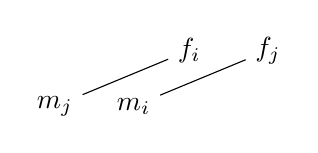
\begin{tikzpicture}[node distance=1cm and 2cm]
\node (fi){$f_i$};
\node [right of=fi] (fj){$f_j$};
\node [below left of=fi] (mi){$m_i$};
\node [left of=mi] (mj){$m_j$};

\path
(fi) edge node {} (mj)
(mi) edge node {} (fj);
\end{tikzpicture}
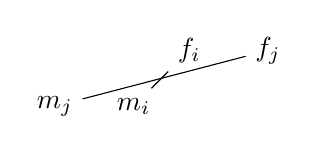
\begin{tikzpicture}[node distance=1cm and 2cm]
\node (fi){$f_i$};
\node [right of=fi] (fj){$f_j$};
\node [below left of=fi] (mi){$m_i$};
\node [left of=mi] (mj){$m_j$};

\path
(fi) edge node {} (mi)
(mj) edge node {} (fj);
\end{tikzpicture}
\end{center}

Regardless of how $m_i,m_j,f_i,f_j$ are paired up, the total distance is the same.  However, in the other configuration, only pairing the sorted elements reduces the total distance, \textit{even if} $f_i$ and $m_i$ are closer, because it avoids "crossing over".
\begin{center}
\begin{tikzpicture}[node distance=1cm and 2cm]
\node (fi){$f_i$};
\node [below right of=fi] (mi) {$m_i$};
\node [above right of=mi] (fj) {$f_j$};
\node [below left of=fi] (mj) {$m_j$};

\path
(fi) edge node {} (mj)
(mi) edge node {} (fj);
\end{tikzpicture}
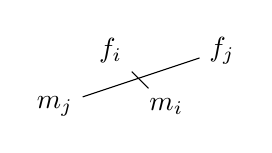
\begin{tikzpicture}[node distance=1cm and 2cm]
\node (fi){$f_i$};
\node [below right of=fi] (mi) {$m_i$};
\node [above right of=mi] (fj) {$f_j$};
\node [below left of=fi] (mj) {$m_j$};

\path
(fi) edge node {} (mi)
(mj) edge node {} (fj);
\end{tikzpicture}
\end{center}

The argument is made much more convincing geometrically.  Once we are convinced of this result, we can write the greedy algorithm very simply.  This algorithm is $O(n\log n + n) = O(n\log n)$.

\begin{problem}

Suppose you have a rod of length $n$, which you can cut into sections.  You can cut up sections of length $i=1,\ldots,n$ inches.  Each different length fetches a different price.  For example:
\begin{center}
\begin{tabular}{c|cccccc}
length $i$ & 1 & 2 & 3 & 4 & 5 & 6 \\
\hline
price $p_i$ & 2 & 3 & 5 & 6 & 7 & 10 \\
\end{tabular}
\end{center}
How can we cut up a rod to maximize profit?
\end{problem}

There are two ways to do this problem.  One is to work from $n$ down to 0, and one is to work from 0 up to $n$.  Both involve trying many different slice combinations to maximize profit.

Using a hash map $m$, the top-down (memoization) solution is given here:
\begin{enumerate}
\item Start at length $n$.
\item We can slice it to lengths $0,1,\ldots,n-1$, each yielding a different amount of profit.
\item Recursively slice until we slice down to length 0.  At this point, return 0.
\item For each rod length, calculate the best price you can get for it by either:
\begin{itemize}
\item Calculating it recursively, considering each slice you can make.
\item Considering where each slice will take you; if the slice takes you to a length already calculated, just look it up in $m$, and add the value of the slice.
\end{itemize}
\item Store the best price for this rod length in $m$.
\item Return the best price for $n$.
\end{enumerate}
As with any memoization solution, this is simply trying every possibility while memorizing subcomputations.  Thus, the code is not far from a brute force solution, but performance is much better.

Using a hash map $m$, the top-down (memoization) solution is given here:
\begin{enumerate}
\item Start at length $n$.
\item We can slice it to lengths $0,1,\ldots,n-1$, each yielding a different amount of profit.
\item Recursively slice until we slice down to length 0.  At this point, return 0.
\item For each rod length, calculate the best price you can get for it by either:
\begin{itemize}
\item Calculating it recursively, considering each slice you can make.
\item Considering where each slice will take you; if the slice takes you to a length already calculated, just look it up in $m$, and add the value of the slice.
\end{itemize}
\item Store the best price for this rod length in $m$.
\item Return the best price for $n$.
\end{enumerate}
As with any memoization solution, this is simply trying every possibility while memorizing subcomputations.  Thus, the code is not far from a brute force solution, but performance is much better.

We can also use dynamic programming:
\begin{enumerate}
\item Start at length $0$.
\item We can arrive here from some higher length \texttt{newLength}.
\item Add that profit to the profit of where you are now.  Call this \texttt{value}.
\begin{itemize}
\item If \texttt{newLength} does not exist in $m$, place it in $m$ with the value \texttt{value}.
\item Otherwise, if \texttt{value} is higher than the current value for \texttt{newLength}, replace it in $m$.
\end{itemize}
\item Return the value for $n$ in $m$.
\end{enumerate}

\begin{problem}
You have three sets of elements, $s_1,s_2,s_3$.  Find all elements in exactly one set.
\end{problem}

We can do this using hash tables.  
\begin{enumerate}
\item Construct hash sets for $s_1,s_2$ and $s_3$.
\item Iterate over $s_1$.  Remove every element in $s_1$ from $s_2$ and $s_3$.
\item Repeat step 2 for $s_2$ and $s_3$.
\item Return the union of $s_1,s_2,s_3$.
\end{enumerate}


\end{document}
